\documentclass[a4paper, titlepage, headings=standardclasses, listof=totoc]{scrartcl}

%\usepackage{plex-serif}
\usepackage{csquotes}
\usepackage[hidelinks]{hyperref}
\usepackage[dutch]{babel}
\usepackage[backend=biber, citestyle=apa, style=apa]{biblatex}
\usepackage{graphicx}
\usepackage{xcolor}
\usepackage[shortlabels]{enumitem}
\usepackage[section]{placeins}
\usepackage{xltabular}
\usepackage{fancyhdr}
\usepackage{pdflscape}
\usepackage{svg}
\usepackage{caption}

% Bibliography.
\addbibresource{../Bibliografie.bib}

% Package used for adding header titles.
\let\origmaketitle\maketitle
\usepackage{titling}
\let\maketitle\origmaketitle

% Flips margins for two-sided prints.
\let\tmp\oddsidemargin
\let\oddsidemargin\evensidemargin
\let\evensidemargin\tmp
\reversemarginpar

% Chapter and title header.
\pagestyle{fancy}
\fancyhead[L]{\textsl{\leftmark}}
\fancyhead[R]{\textsc{\thetitle}}
\renewcommand{\footrulewidth}{0.4pt}

% Complementary colors to the red color from the HAN logo.
\definecolor{hanA}{HTML}{D91E57}
\definecolor{hanB}{HTML}{8C062E}
\definecolor{hanC}{HTML}{D9CD34}
\definecolor{hanD}{HTML}{09A9D9}
\definecolor{hanE}{HTML}{0D6F8C}

% Coloring elements.
%\let\HeadRule\headrule
%\let\FootRule\footrule
%\renewcommand\headrule{\color{hanE}\HeadRule}
%\renewcommand\footrule{\textcolor{hanE}\FootRule}
%\addtokomafont{section}{\color{hanA}}
%\addtokomafont{subsection}{\color{hanA}}
%\addtokomafont{subsubsection}{\color{hanA}}
%\let\oldtextbf\textbf
%\renewcommand{\textbf}[1]{\textcolor{hanB}{\oldtextbf{#1}}}

% Fonts.
%\renewcommand{\rmdefault}{bch}
\renewcommand{\rmdefault}{bch}
\renewcommand{\sfdefault}{qag}

% Custom commands and environments.
% Itemize without vertical spacing.
\newenvironment{smallitemize}{\begin{itemize}[nosep,after=\strut]}{\end{itemize}}
% Enumerate without vertical spacing.
\newenvironment{smallenumerate}{\begin{enumerate}[nosep,after=\strut]}{\end{enumerate}}
% Minipage made to look like a floating figure.
\newenvironment{mpfigure}{\vspace{\floatsep}\noindent\begin{minipage}{\linewidth}\captionsetup{type=figure}}{\end{minipage}\vspace{1.1\floatsep}}
\newcommand{\comment}[1]{}

% Custom title page entries.
\def\Version#1{\def\version{#1}}
\def\Subtitle#1{\def\csubtitle{#1}}
\def\Teacher#1{\def\teacher{#1}}

% Other settings.
\setlength{\LTpre}{0pt}

\title{Software Design Description}
\Subtitle{OOSE OOAD casus - Quebble}
\Teacher{Marco Engelbart}
\Version{1}

\begin{document}

\begin{titlepage}
    \sffamily
    \begin{center}
    \vspace*{1cm}

    \color{hanA}\huge\textbf{\thetitle}
    
    \vspace{0.5cm}

    \color{hanB}\Large \csubtitle

    \vspace{1.5cm}\color{black}

    Sjoerd Scheffer

    \vspace{0.1cm}

    579392

    \vfill

    \includesvg{../Afbeeldingen/logo.svg}

    \vspace{2.0cm}\large

    Docent: \teacher

    \vspace{1.0cm}\normalsize

    \today

    \vspace{0.5cm}

    Versie \version
    
    \end{center}
\end{titlepage}
\cleardoublepage
\tableofcontents
\clearpage
\listoftables
\listoffigures
\clearpage


\clearpage\section{Inleiding}
%Introduction

\subsection{Algemene beschrijving}
%Overall description <Provide a short description of the software being specified and its purpose, including relevant benefits, objectives, and goals. If a separate description of the product scope is available (e.g. in the PvA or SRS), place a link here rather than duplicating its contents here.>
\textit{Zie de Software Requirements Specification.}

\subsection{Doel van dit document}
%Purpose of this document <Full description of the main objectives of the SDD document.>
Dit document beschrijft de technische vertaling van de uitgewerkte usecases uit het Software Requirements Specification. Dit document beschrijft het ontwerp van Quebble als opgesteld aan de hand van de casusopdracht.

%\subsection{Definities, acroniemen en afkortingen}
%Definitions, acronyms and abbreviations Table consisting of colums Term, Description.

%\clearpage\section{Architectuuroverzicht}
%Architectural overview <Provide a high level overview of the architectural design, for instance by means of an architectural sketch. Make sure you show at least all sub-systems, and links to external systems. The sketch can be informal. The use of UML is not required.>

\clearpage\section{Gedetailleerde ontwerpbeschrijving}
%Detailed design description <This section contains detailed design documentation of all software components. The content of this section grows iteratively during the sprints. At the end of each sprint, the diagrams shown need to be consistent.>

%\subsection{Deploymentdiagram}
%Deployment diagram <Provide a UML deployment diagram showing all physical and virtual nodes used in the system. The diagram must also contain all deployment artifacts used in the system, for instance JAR or WAR files, or web artifacts.>

%\subsubsection{Deployment gerelateerde ontwerpbeslissingen}
%Design decisions related to deployment <Describe all design decisions manifested in the deployment diagram. For instance the choice of operating systems, protocols, distribution of components over sub-systems and the like.>

\subsection{Ontwerp subsysteem Quebble}
%Design subsystem A <Do not really name the section “Sub-System A”, use a name that describes the responsibility of the sub-system, instead. Provide a section for each sub-system. These sections are iteratively added and refined during the sprints. Examples of sub-systems include Persistent Storage, Business Tier, Web Application, Webservice API. The sub-sections below may be extended if you think this is useful for describing the software design. The sub-sections below are only required for object-oriented sub-systems. Use other means to describe non-OO sub-systems (for instance Javascript modules).>

\subsubsection{Klassendiagram}
%Design class diagram<Object-oriented sub-systems should be described using a class diagram. If classes or interfaces are used across sub-systems, make sure you mention this in the description of the class diagrams. If your system entails layers, make sure you indicate this in the class diagram, e.g. by means of packages. For each class diagram, make sure you also mention the deployment artifact (from the deployment diagram) it is part of.>
Deze sectie bevat het klassendiagram. Deze is gebaseerd op het domeinmodel uit de Software Requirements Specification. Daarop volgt een toelichting voor de afwijkingen van het domeinmodel.

\begin{mpfigure}
    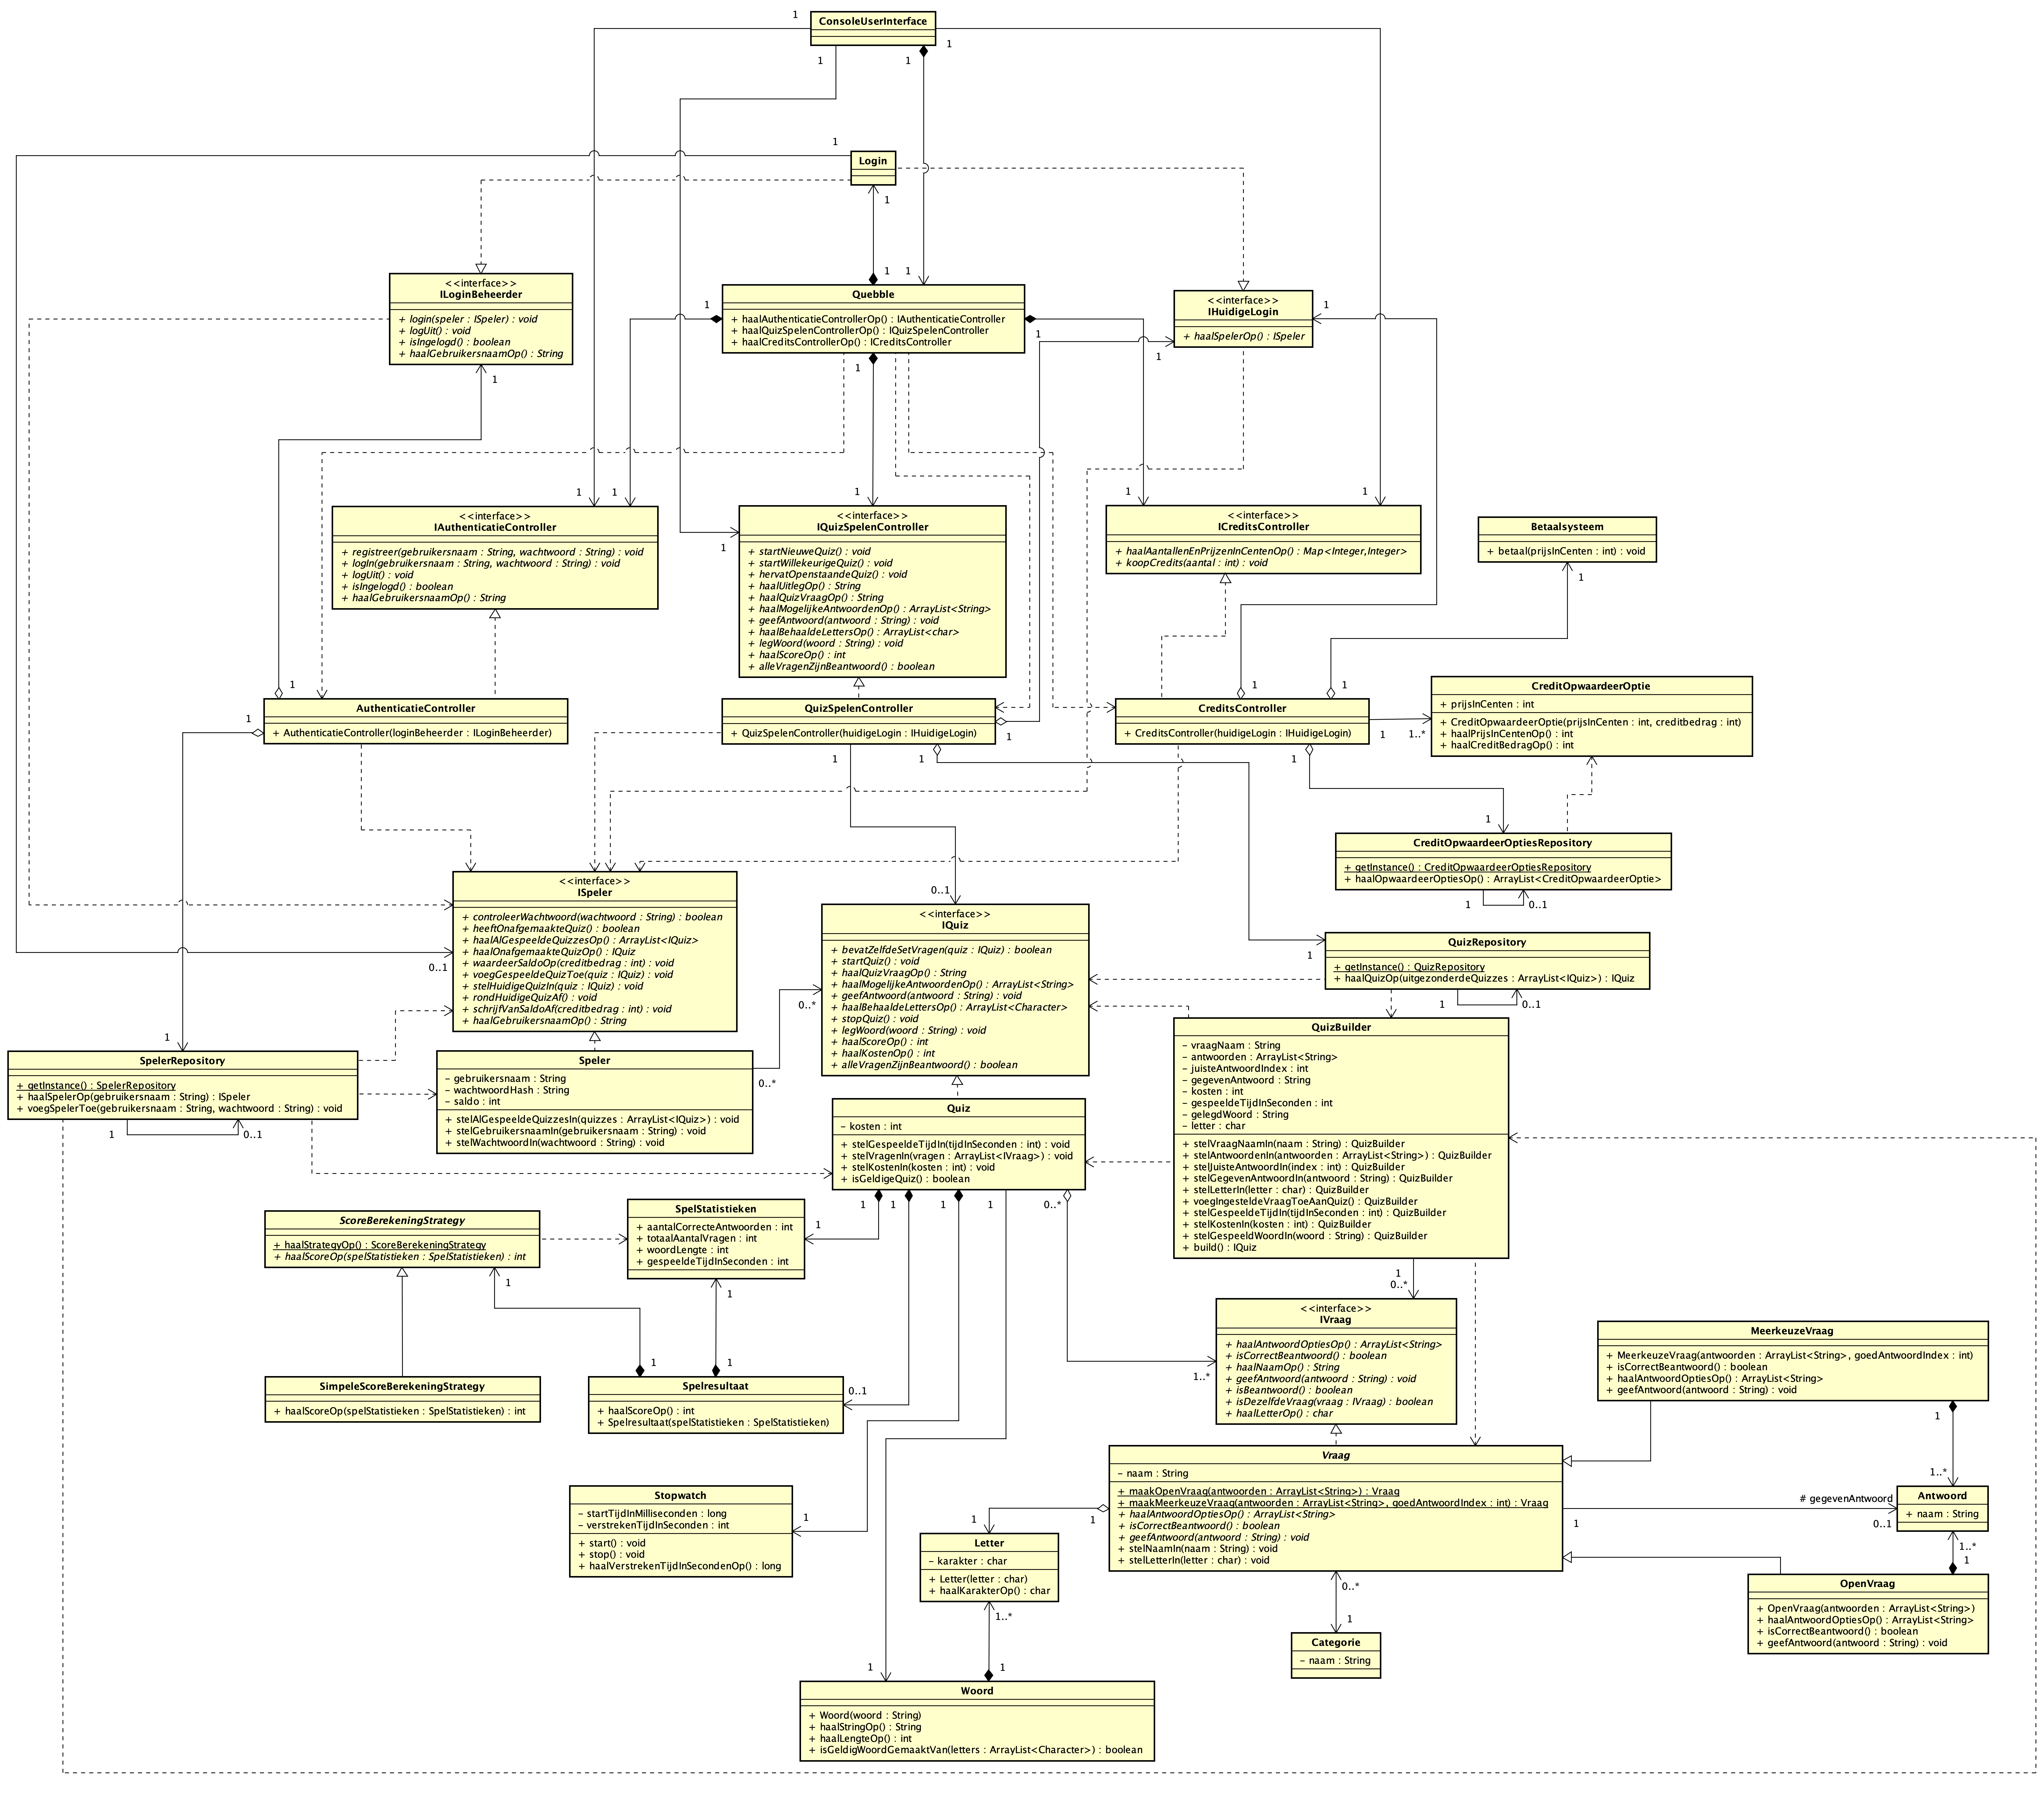
\includegraphics[width=\linewidth]{../Afbeeldingen/Klassendiagram.png}
    \caption{Klassendiagram}
    \label{fig:klassendiagram}
\end{mpfigure}

\noindent\begin{minipage}{\linewidth}
    De gebruikte patterns en principes uit tabel \ref{tab:solid}, \ref{tab:gof} en \ref{tab:grasp} van sectie \ref{sec:designdesicions} zorgen voor verschillen met het domeinmodel uit de Software Rquirements Specification. Daarnaast zijn er nog een aantal verschillen:
    \begin{itemize}
        \item De associatie tussen aan de ene kant \textbf{Speler} en aan de andere kant \textbf{Antwoord}, \textbf{Vraag} en \textbf{Woord}. Dit ten behoeve van het GRASP-principe Low Coupling en het daarbij toegepaste pattern Indirection (\cite{larman}).
        \item Het attribuut \textit{goed} van \textbf{Antwoord}. Dit attribuut bestaat niet in het klassendiagram omdat de verantwoordelijkheid voor de goedkeuring bij de \textbf{Vraag} ligt. Anders zouden er bijvoorbeeld meerdere goede antwoorden bij een meerkeuzevraag kunnen zitten.
        \item De klasse \textbf{Creditbedrag}. Dit is een refactoring omdat het object geen verantwoordelijkheid had naast het bijhouden van een enkel aantal credits (\cite{inlineclass}). De klasse veroorzaakte alleen maar rommeligheid in het ontwerp.
        \item Alle klassen in het klassendiagram die geen dependency/associatie zijn van QuizController. Het domeinmodel beschrijft alleen de concepten voor het spelen van een quiz.
    \end{itemize}
\end{minipage}

\subsubsection{Sequencediagrammen}
%Sequence diagrams <Provide sequence diagrams for major object interactions within the sub-system.  It is ok if sequence diagrams cross sub-system boundaries. Make sure you explain this in the description of the diagram. Sequence diagrams must be consistent with the class diagrams described above. Also, if sequence diagrams cover interaction with users, make sure the diagrams are consistent with SDDs you may have documented as part of the SRS.>
Deze sectie bevat sequence diagrammen die de belangrijkste systeemoperaties laten zien van de uitgewerkte usecases van de Software Requirements Specification.

\begin{mpfigure}
    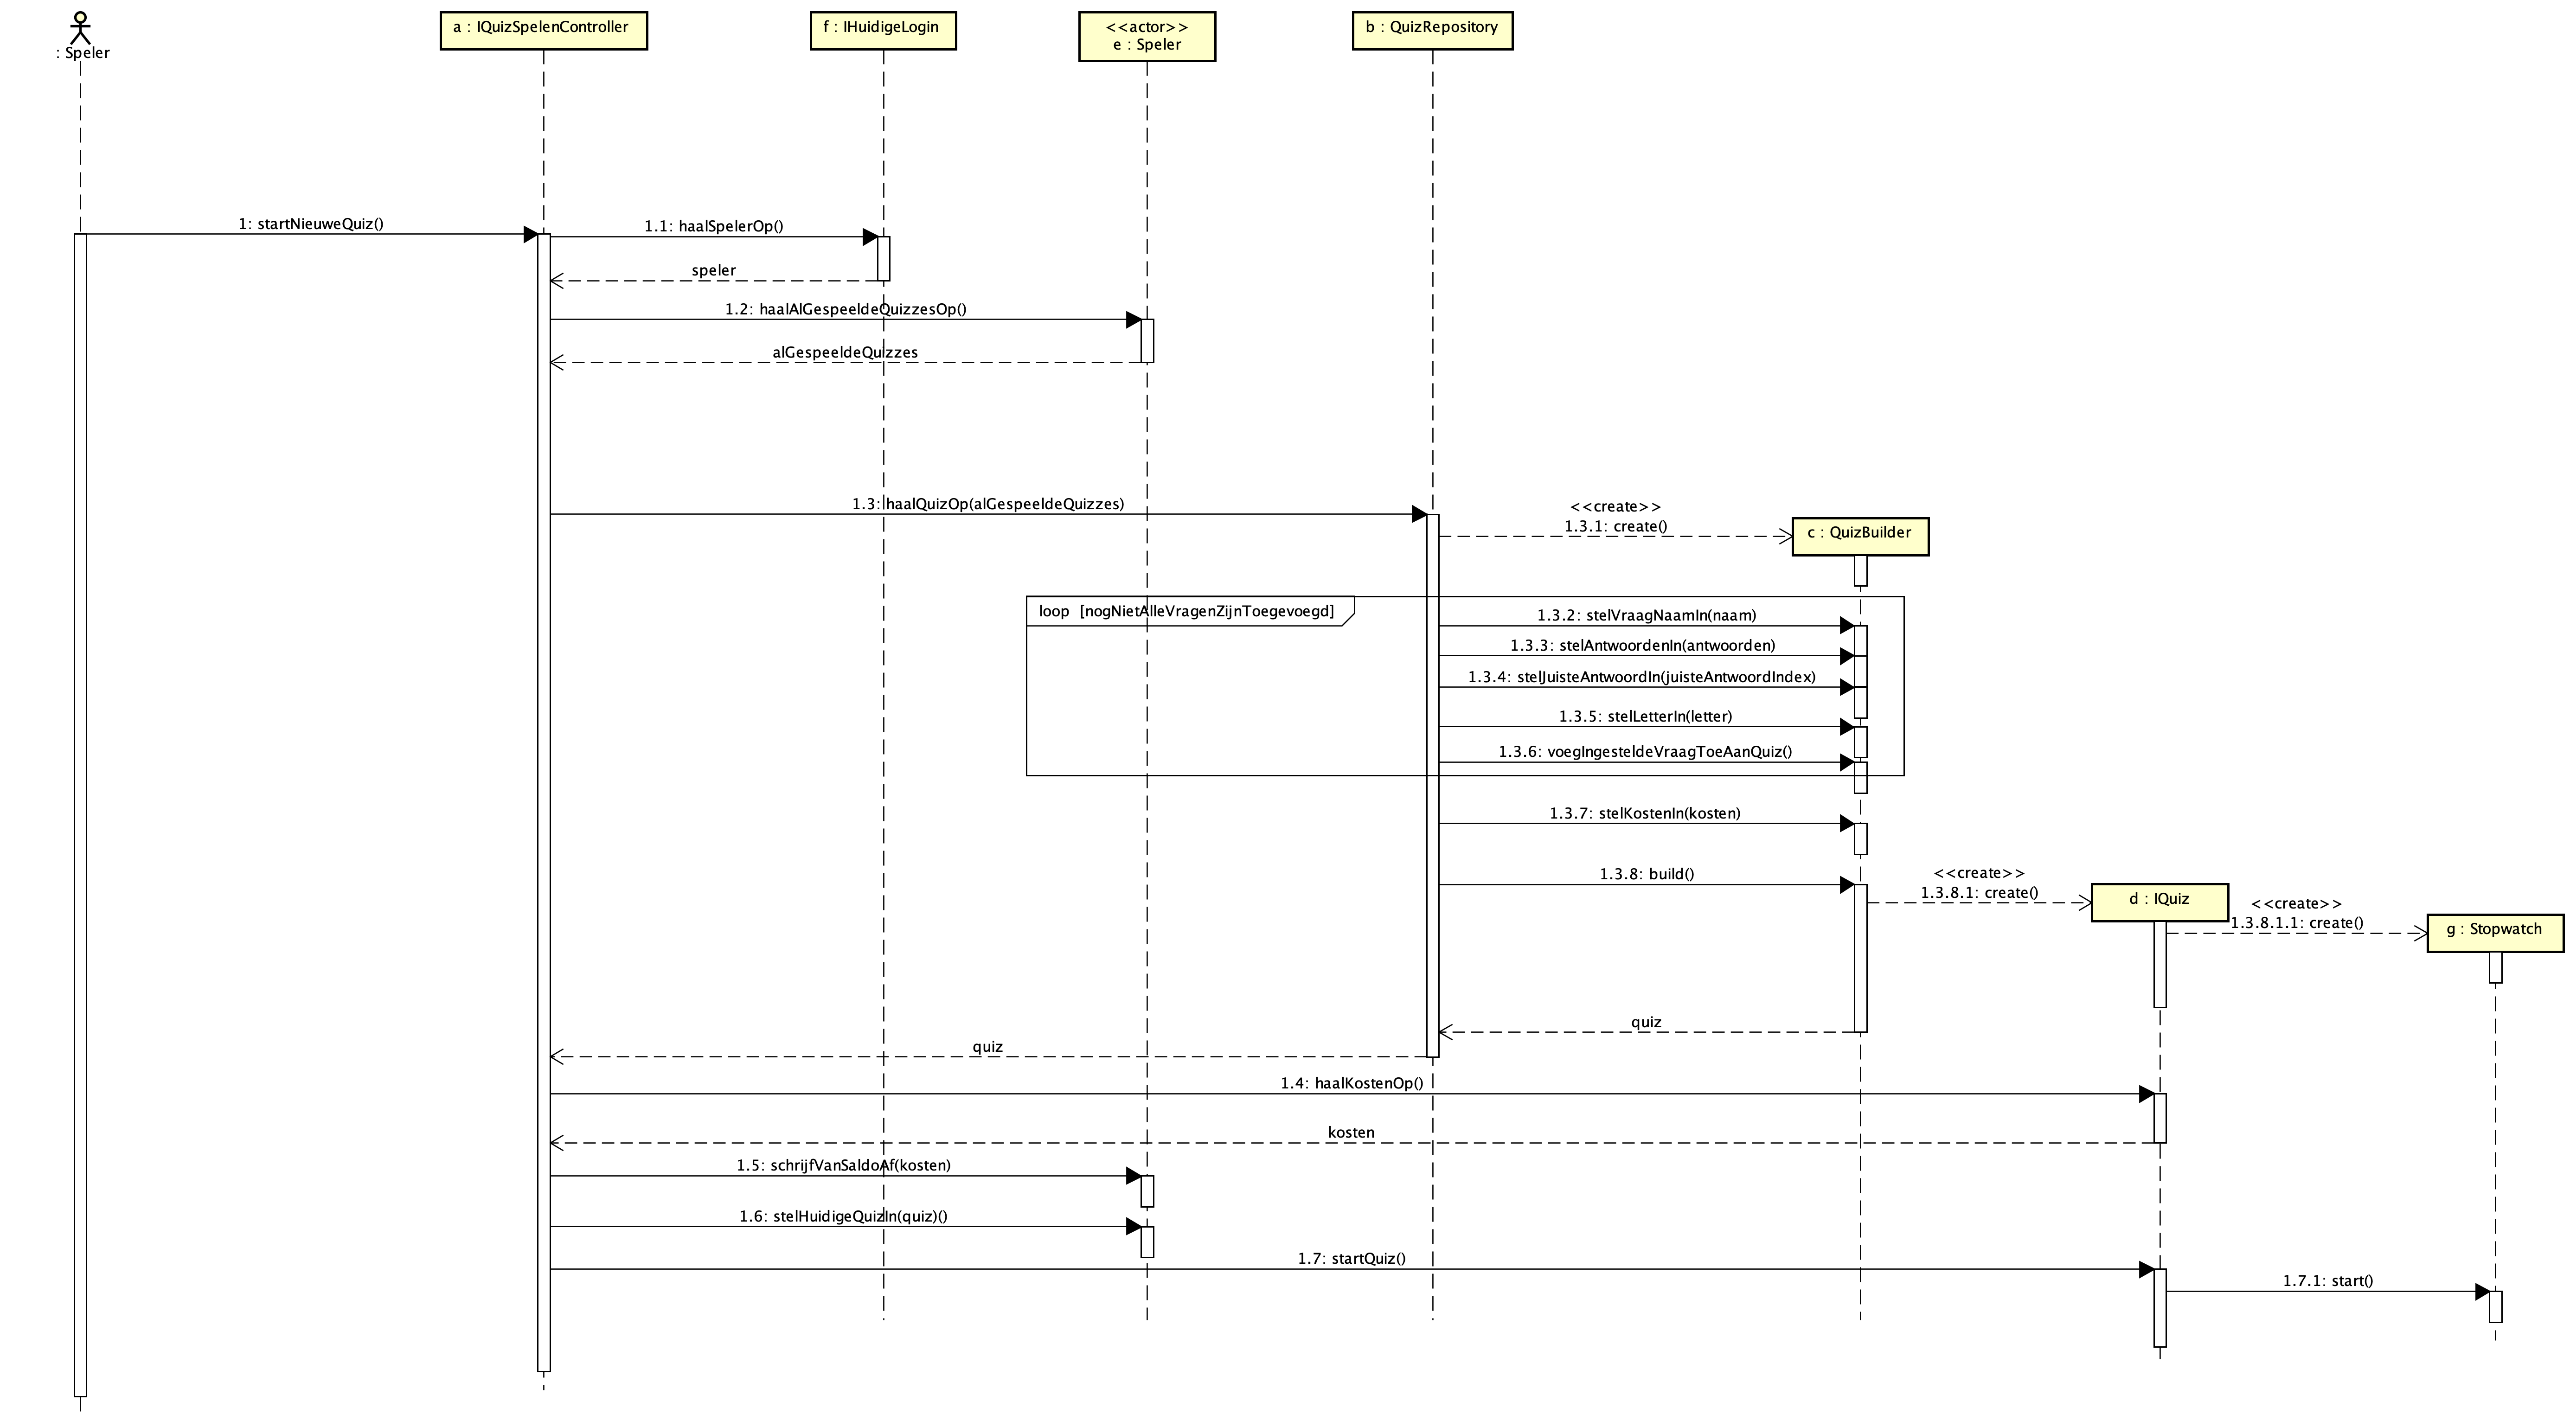
\includegraphics[width=\linewidth]{../Afbeeldingen/Sequence diagrammen/startNieuweQuiz.png}
    \caption{Sequencediagram voor systeemoperatie \textit{startNieuweQuiz}}
    \label{fig:startnieuwequiz}
\end{mpfigure}

\begin{mpfigure}
    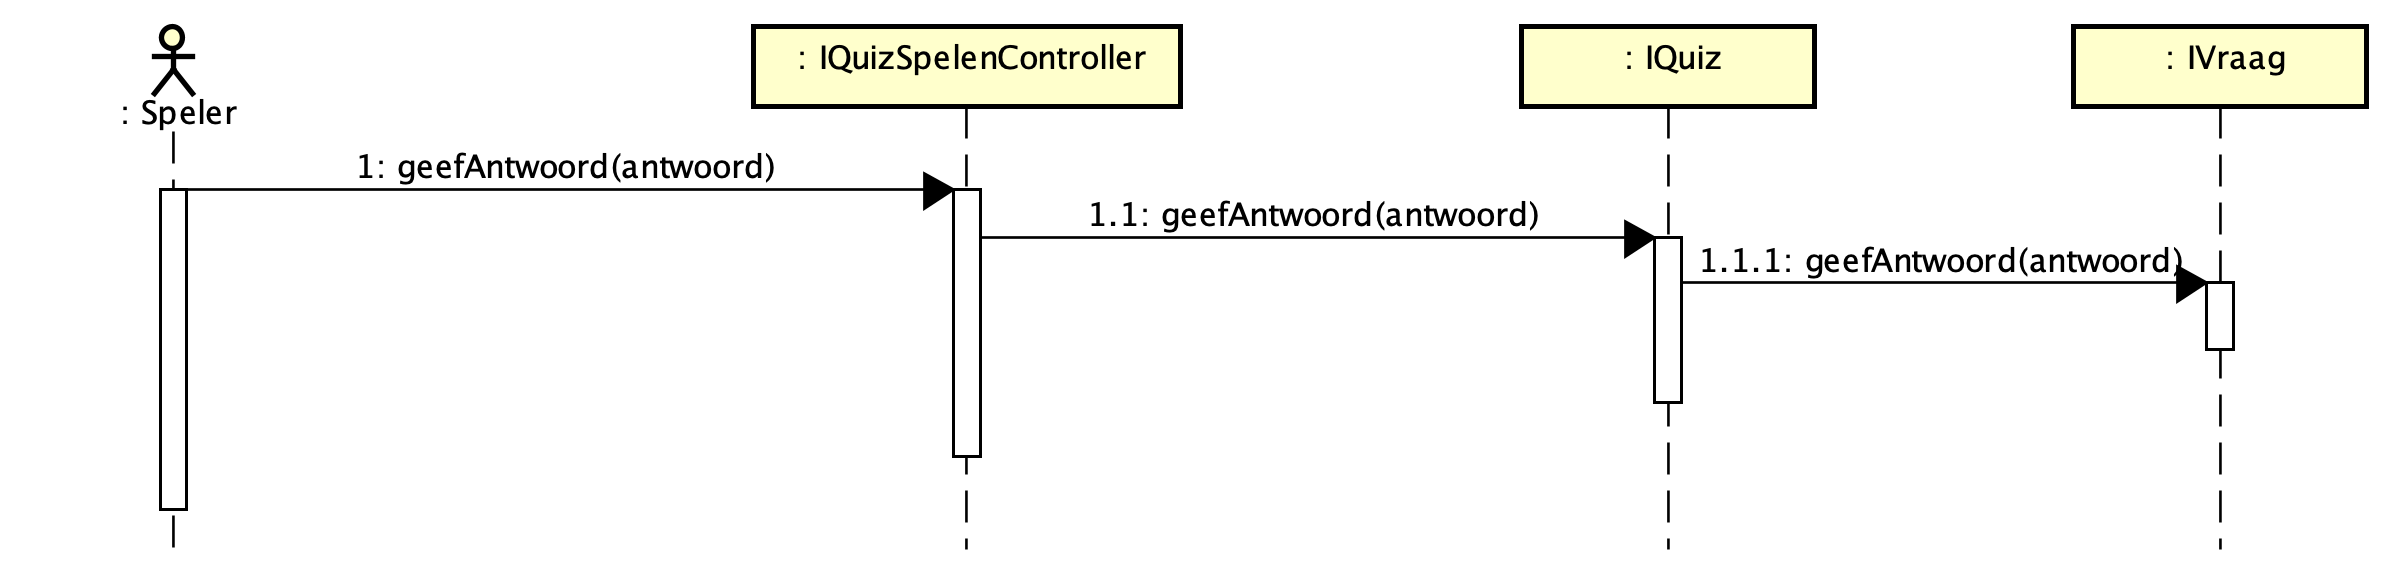
\includegraphics[width=\linewidth]{../Afbeeldingen/Sequence diagrammen/geefAntwoord.png}
    \caption{Sequencediagram voor systeemoperatie \textit{geefAntwoord}}
    \label{fig:geefantwoord}
\end{mpfigure}

\begin{mpfigure}
    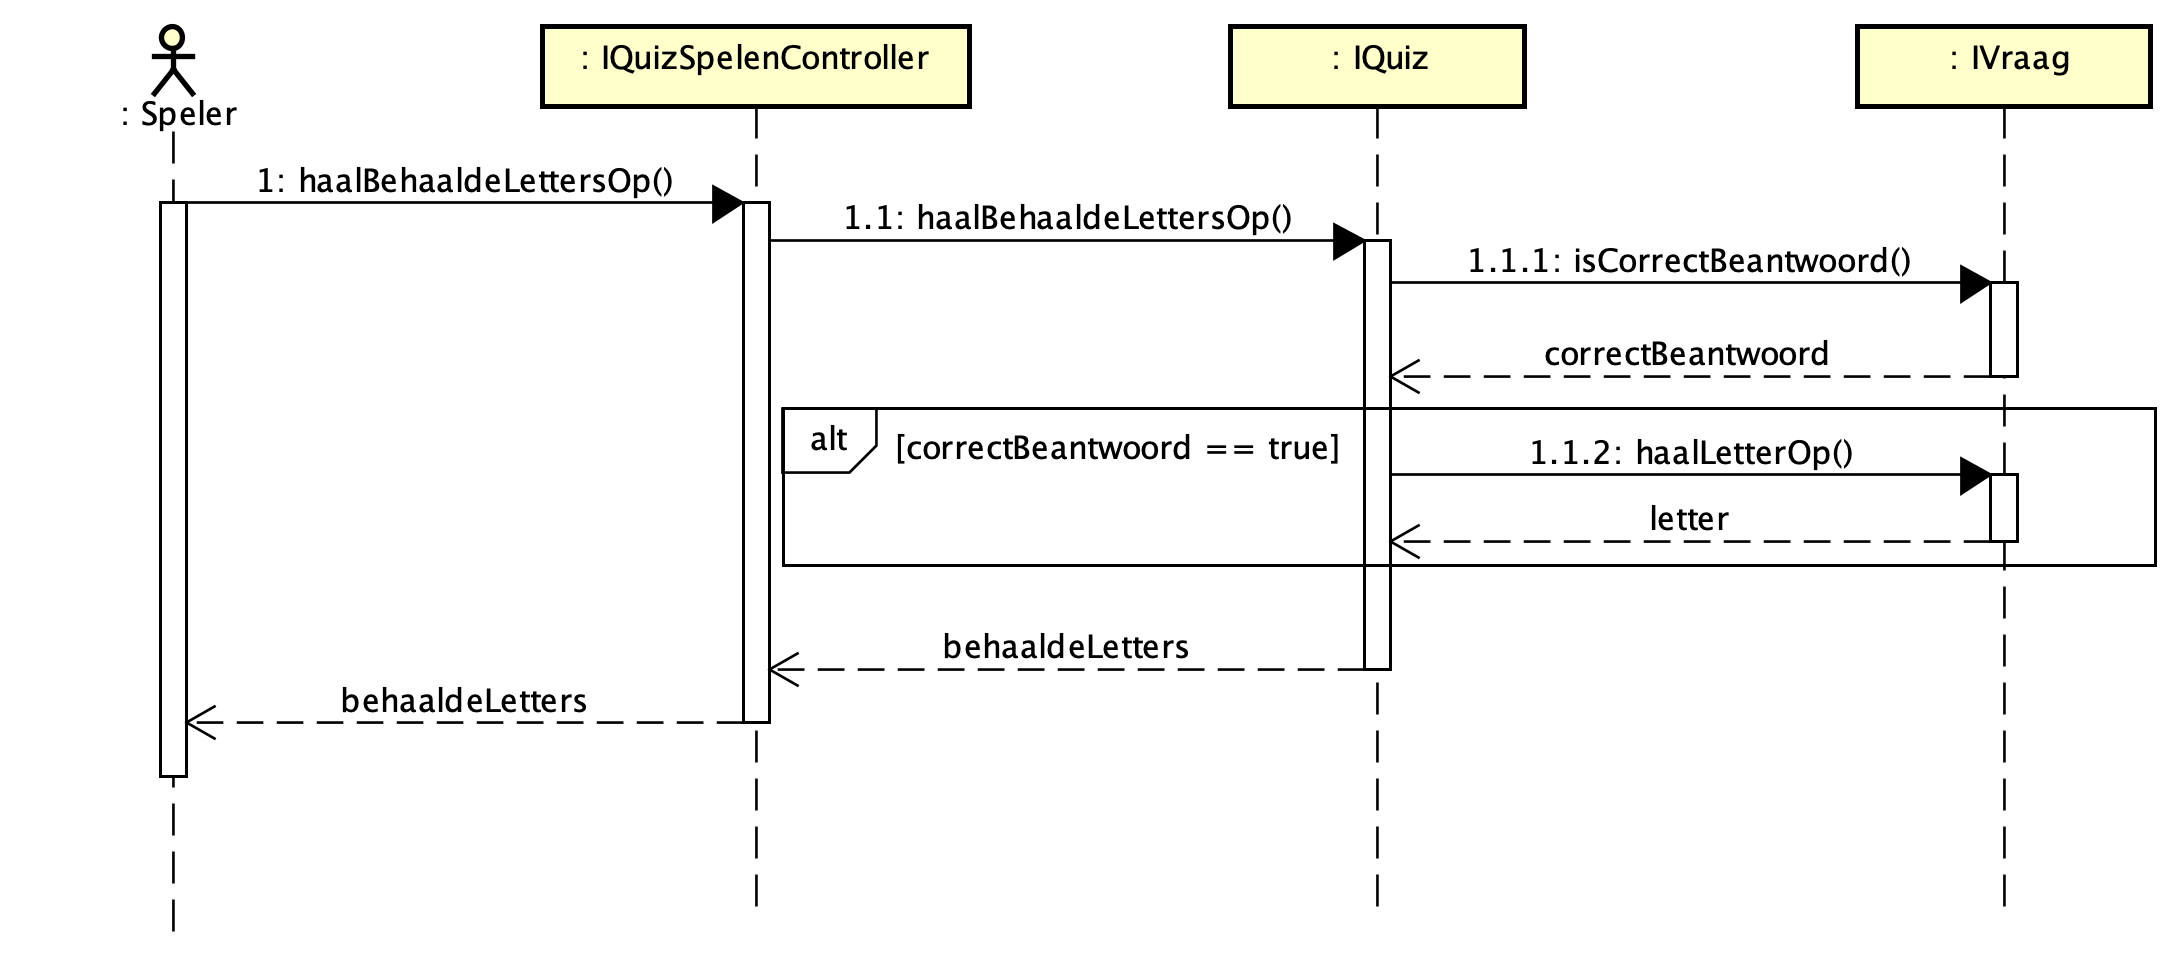
\includegraphics[width=\linewidth]{../Afbeeldingen/Sequence diagrammen/haalBehaaldeLettersOp.png}
    \caption{Sequencediagram voor systeemoperatie \textit{haalBehaaldeLettersOp}}
    \label{fig:haalbehaaldelettersop}
\end{mpfigure}

\begin{mpfigure}
    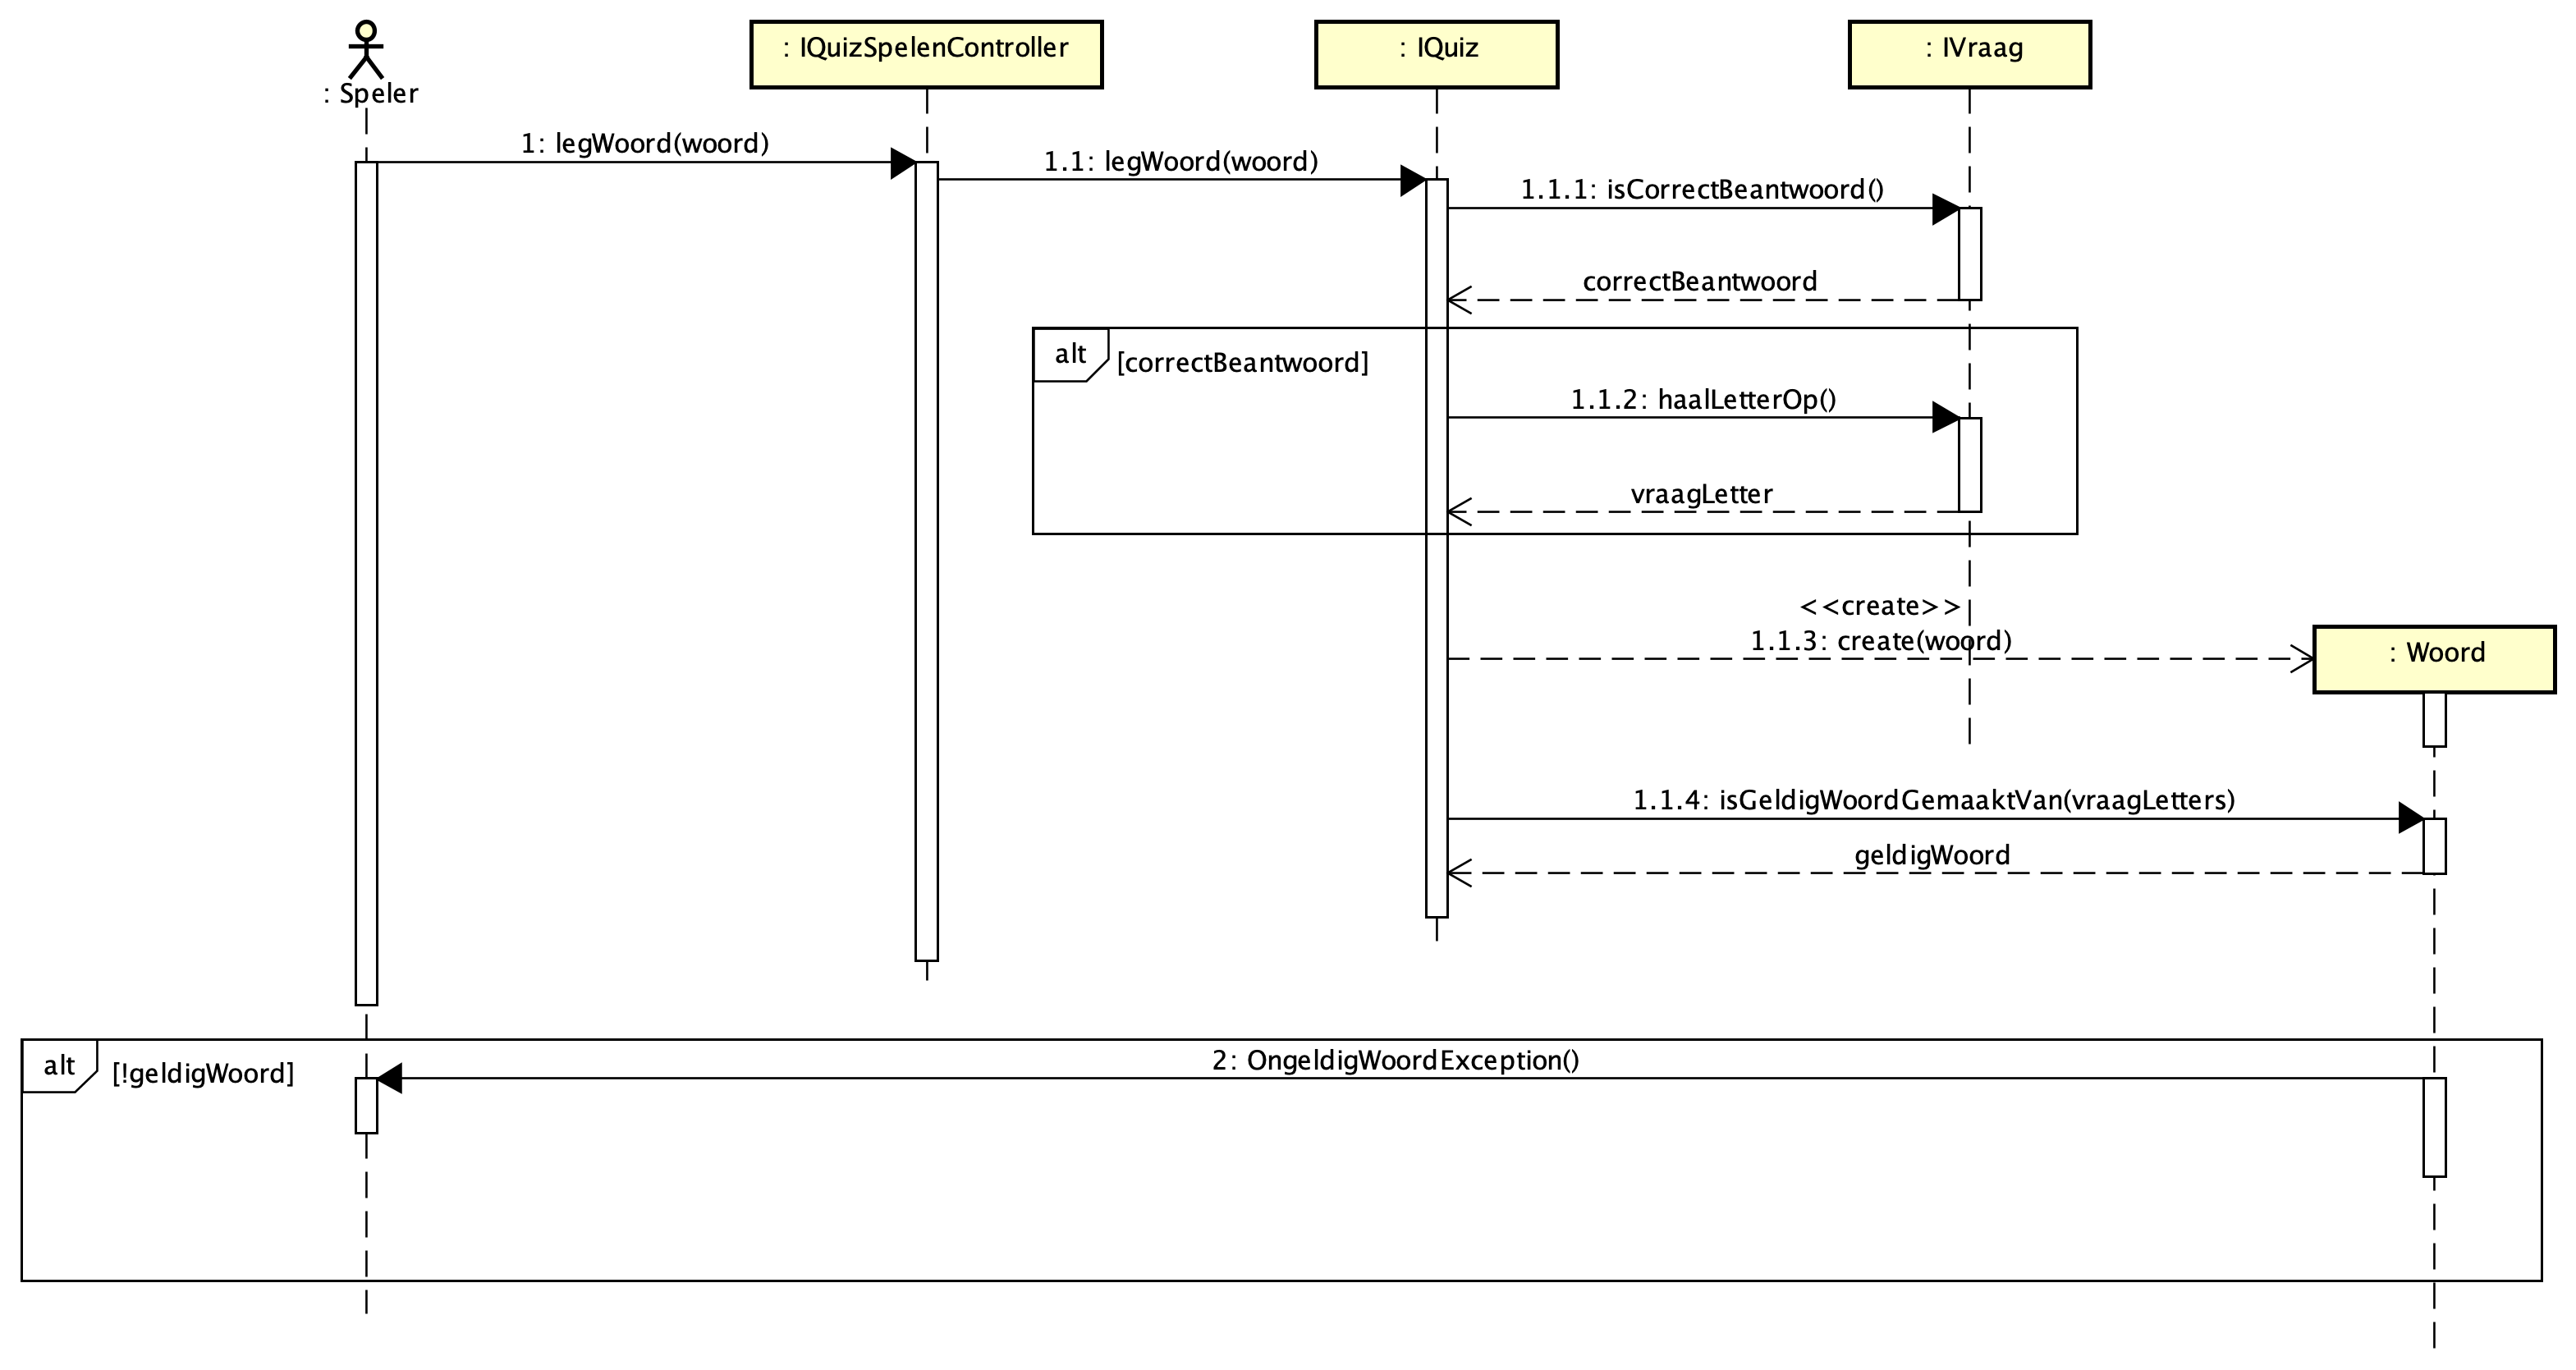
\includegraphics[width=\linewidth]{../Afbeeldingen/Sequence diagrammen/legWoord.png}
    \caption{Sequencediagram voor systeemoperatie \textit{legWoord}}
    \label{fig:legwoord}
\end{mpfigure}

\begin{mpfigure}
    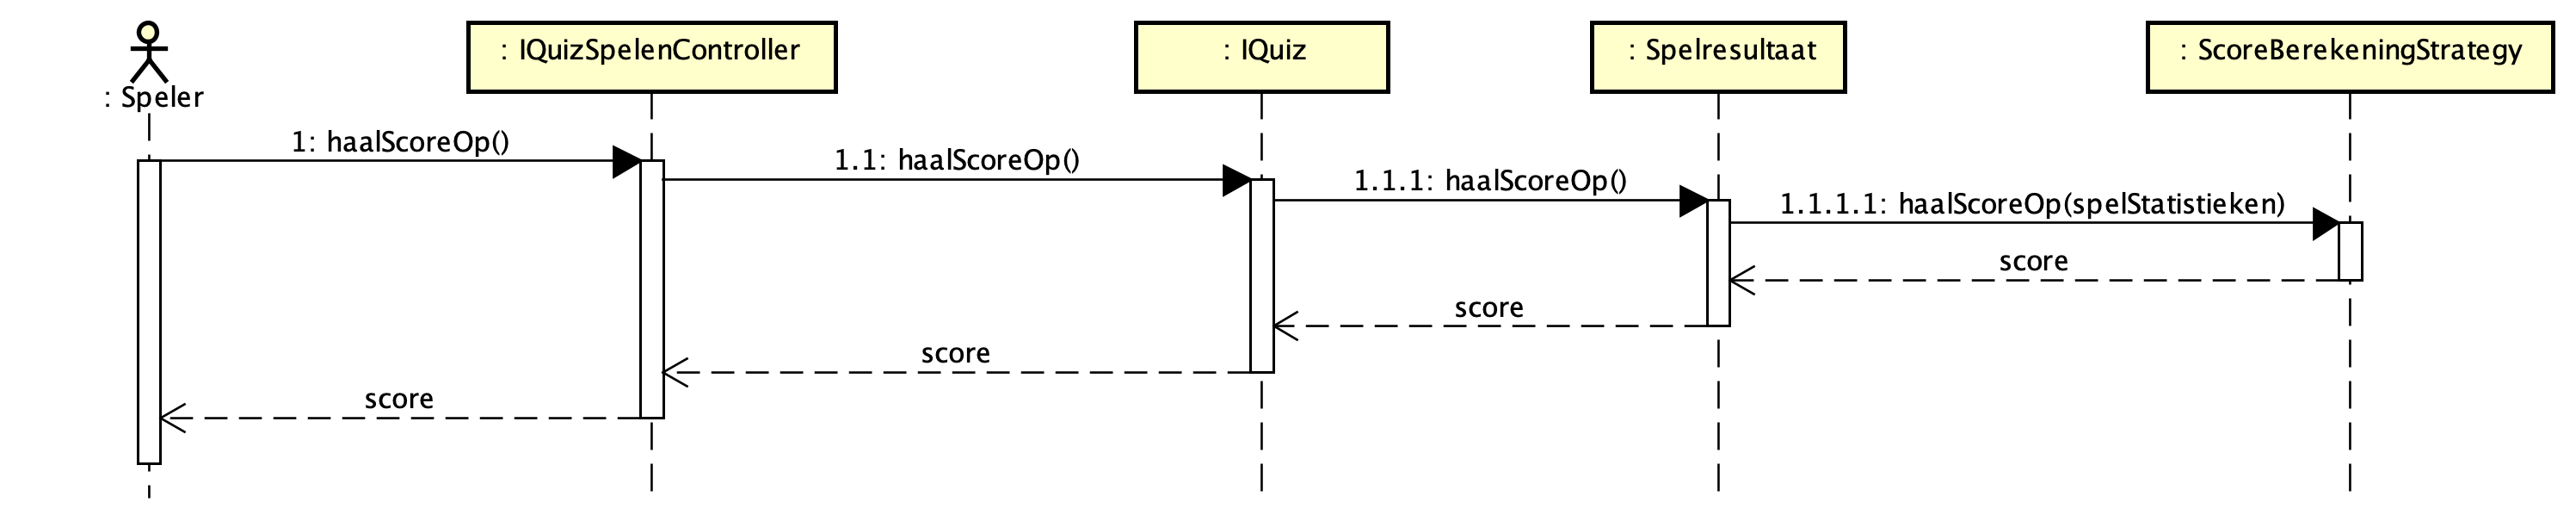
\includegraphics[width=\linewidth]{../Afbeeldingen/Sequence diagrammen/haalScoreOp.png}
    \caption{Sequencediagram voor systeemoperatie \textit{haalScoreOp}}
    \label{fig:haalscoreop}
\end{mpfigure}

\begin{mpfigure}
    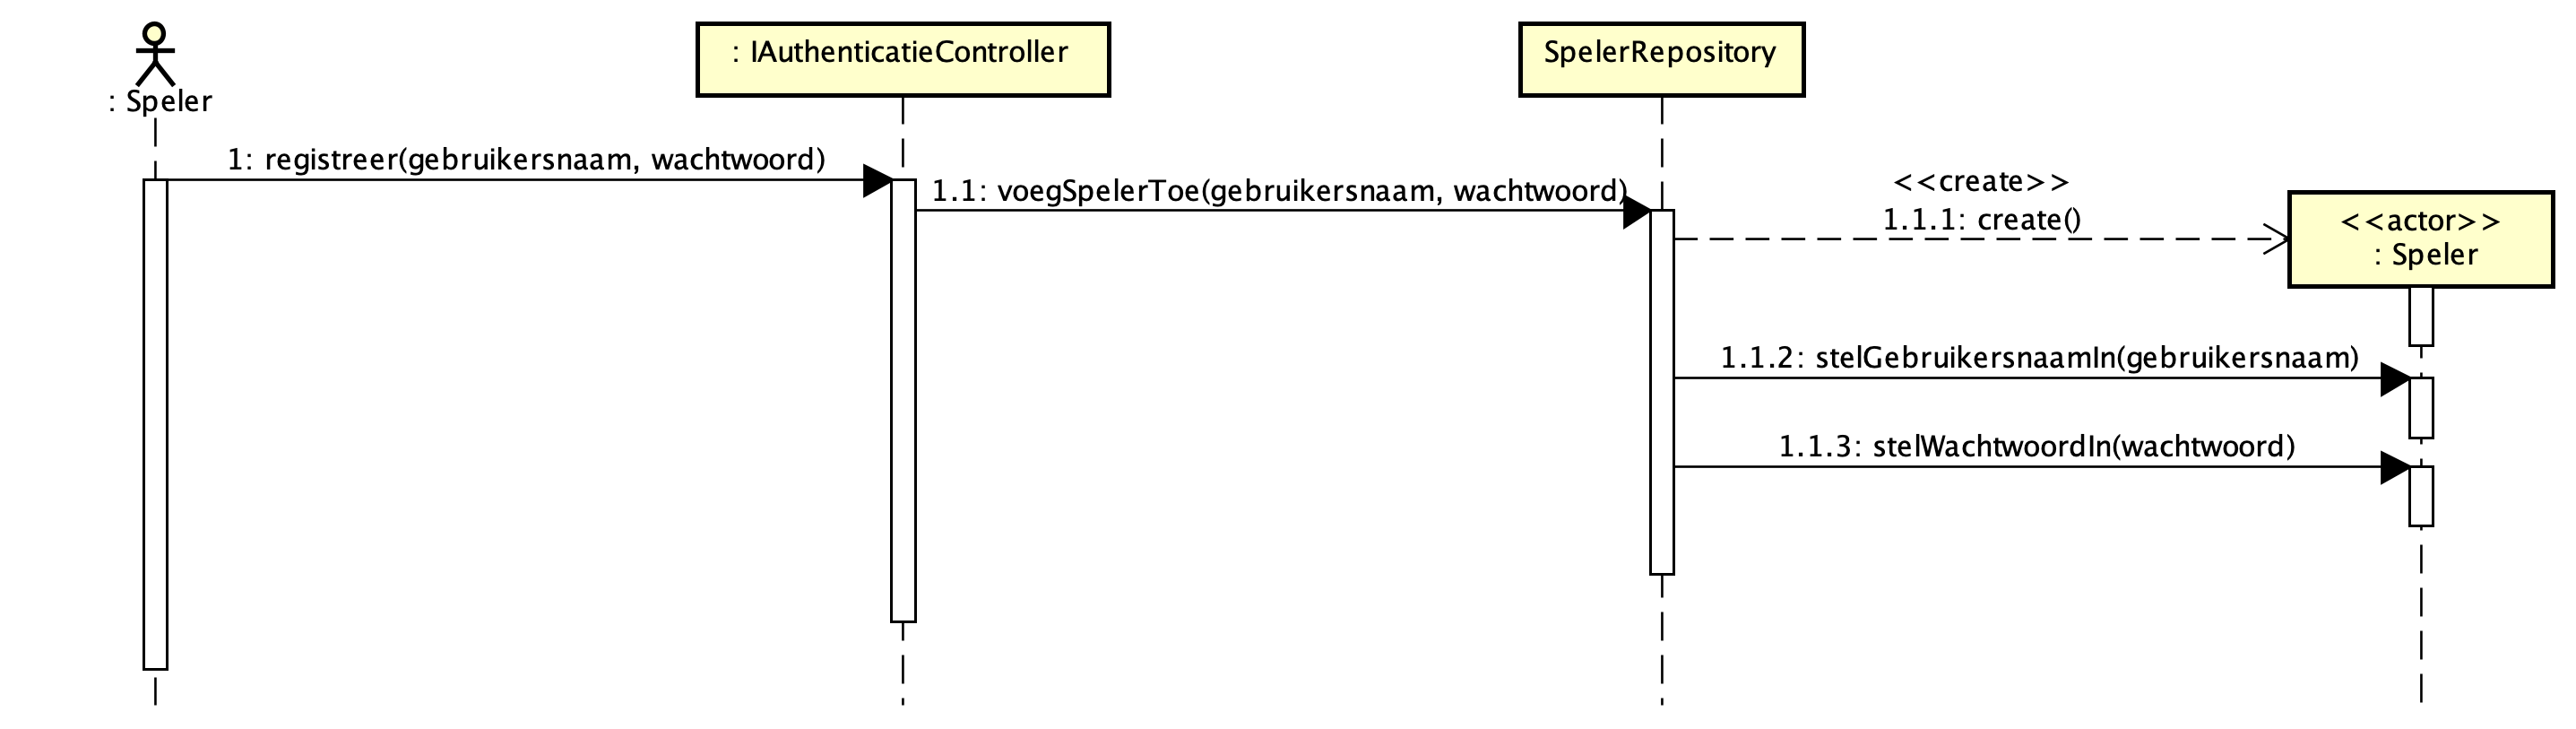
\includegraphics[width=\linewidth]{../Afbeeldingen/Sequence diagrammen/registreer.png}
    \caption{Sequencediagram voor systeemoperatie \textit{registreer}}
    \label{fig:registreer}
\end{mpfigure}

\begin{mpfigure}
    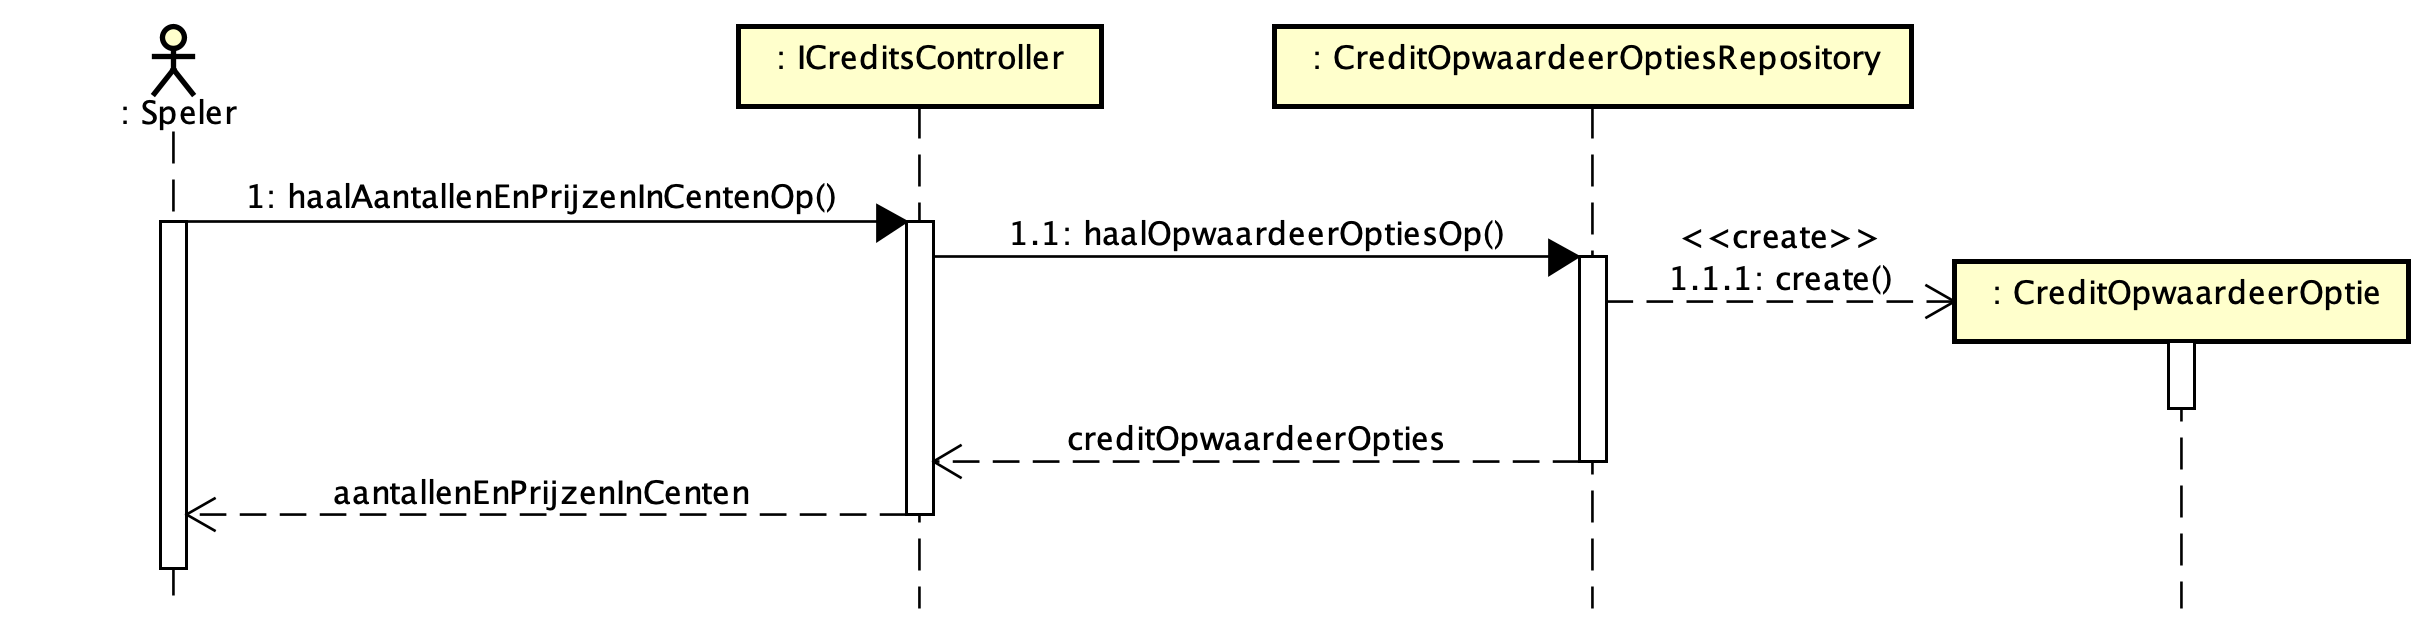
\includegraphics[width=\linewidth]{../Afbeeldingen/Sequence diagrammen/haalAantallenEnPrijzenInCentenOp.png}
    \caption{Sequencediagram voor systeemoperatie \textit{haalAantallenEnPrijzenInCentenOp}}
    \label{fig:haalaantallenenprijzenincentenop}
\end{mpfigure}

\begin{mpfigure}
    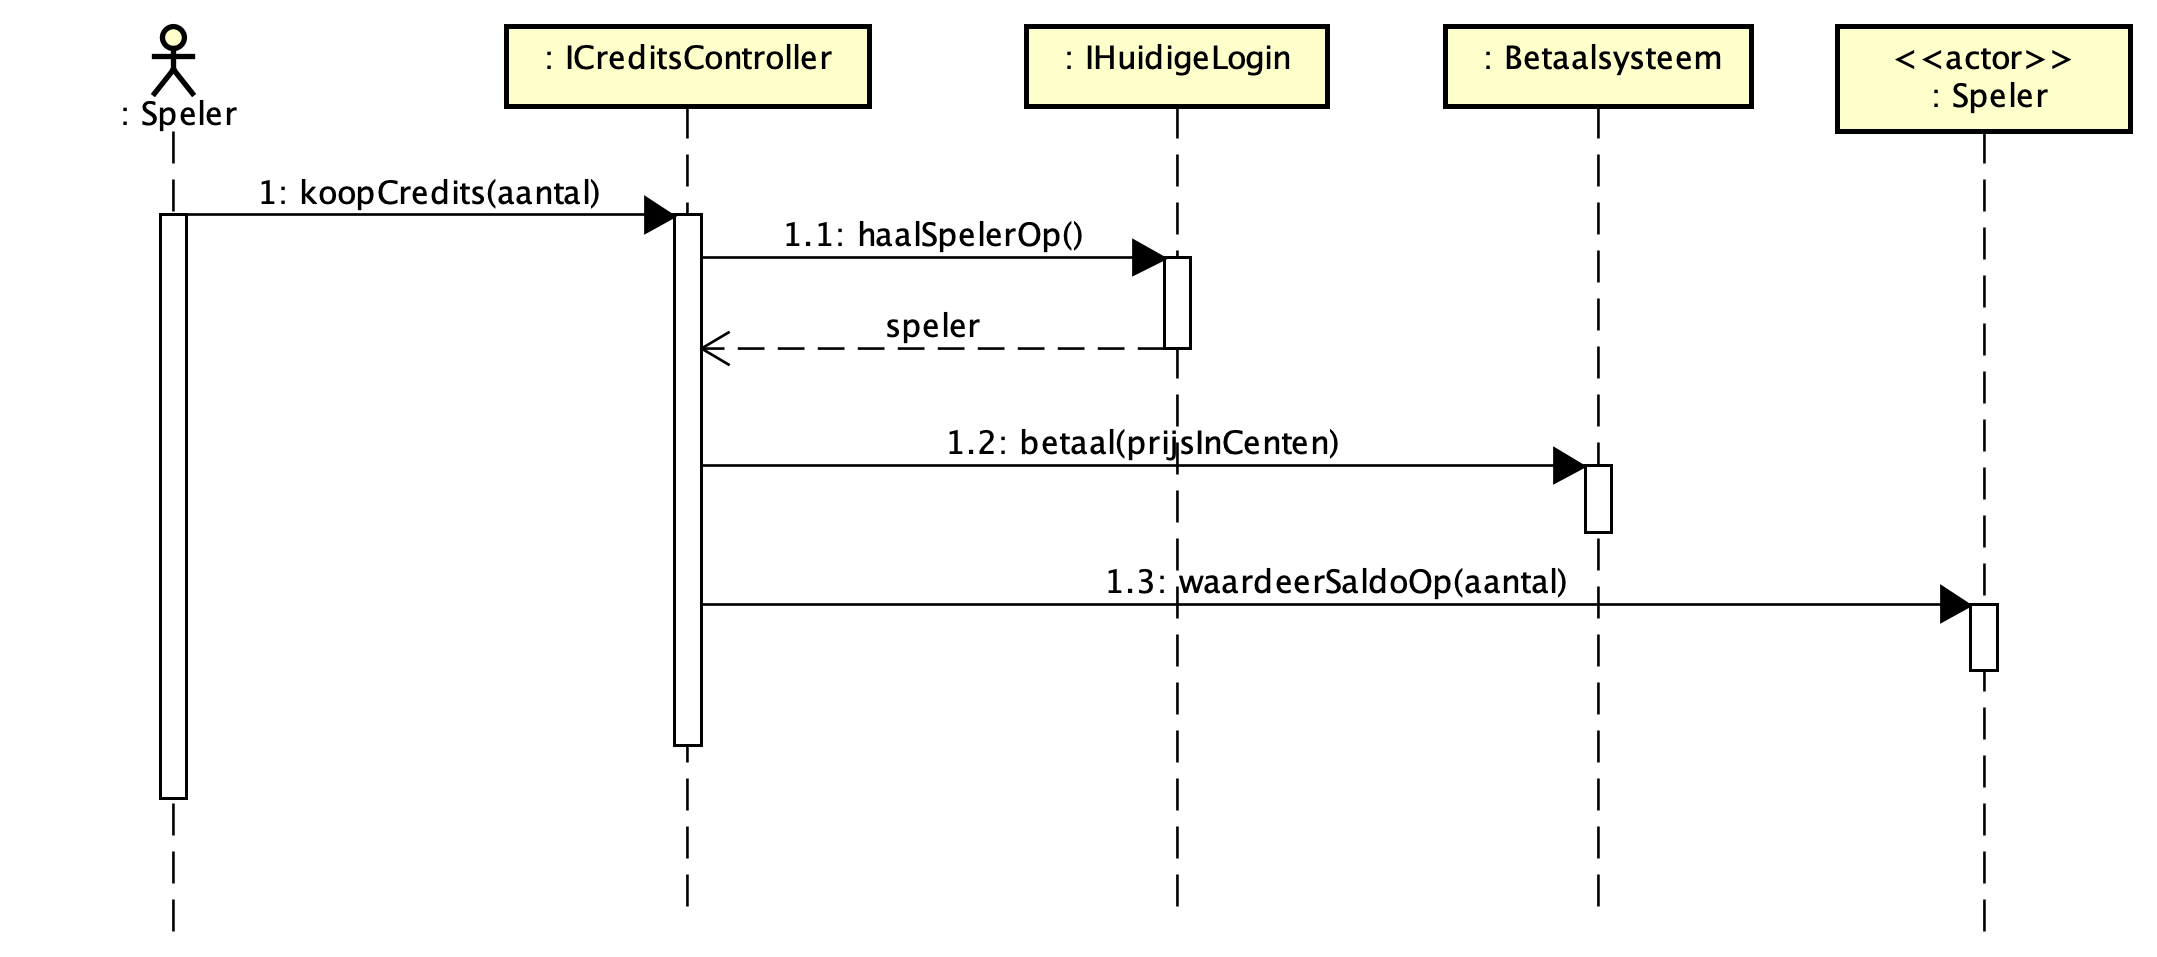
\includegraphics[width=\linewidth]{../Afbeeldingen/Sequence diagrammen/koopCredits.png}
    \caption{Sequencediagram voor systeemoperatie \textit{koopCredits}}
    \label{fig:koopcredits}
\end{mpfigure}

\subsubsection{Activity- en statediagrammen}
%Activity and state diagrams <This section is optional. If useful, provide activity and/or state diagrams to describe complex work flows and system state transitions>
Deze sectie bevat een activitydiagram voor de usecase \textit{Quiz spelen}.

\begin{mpfigure}
    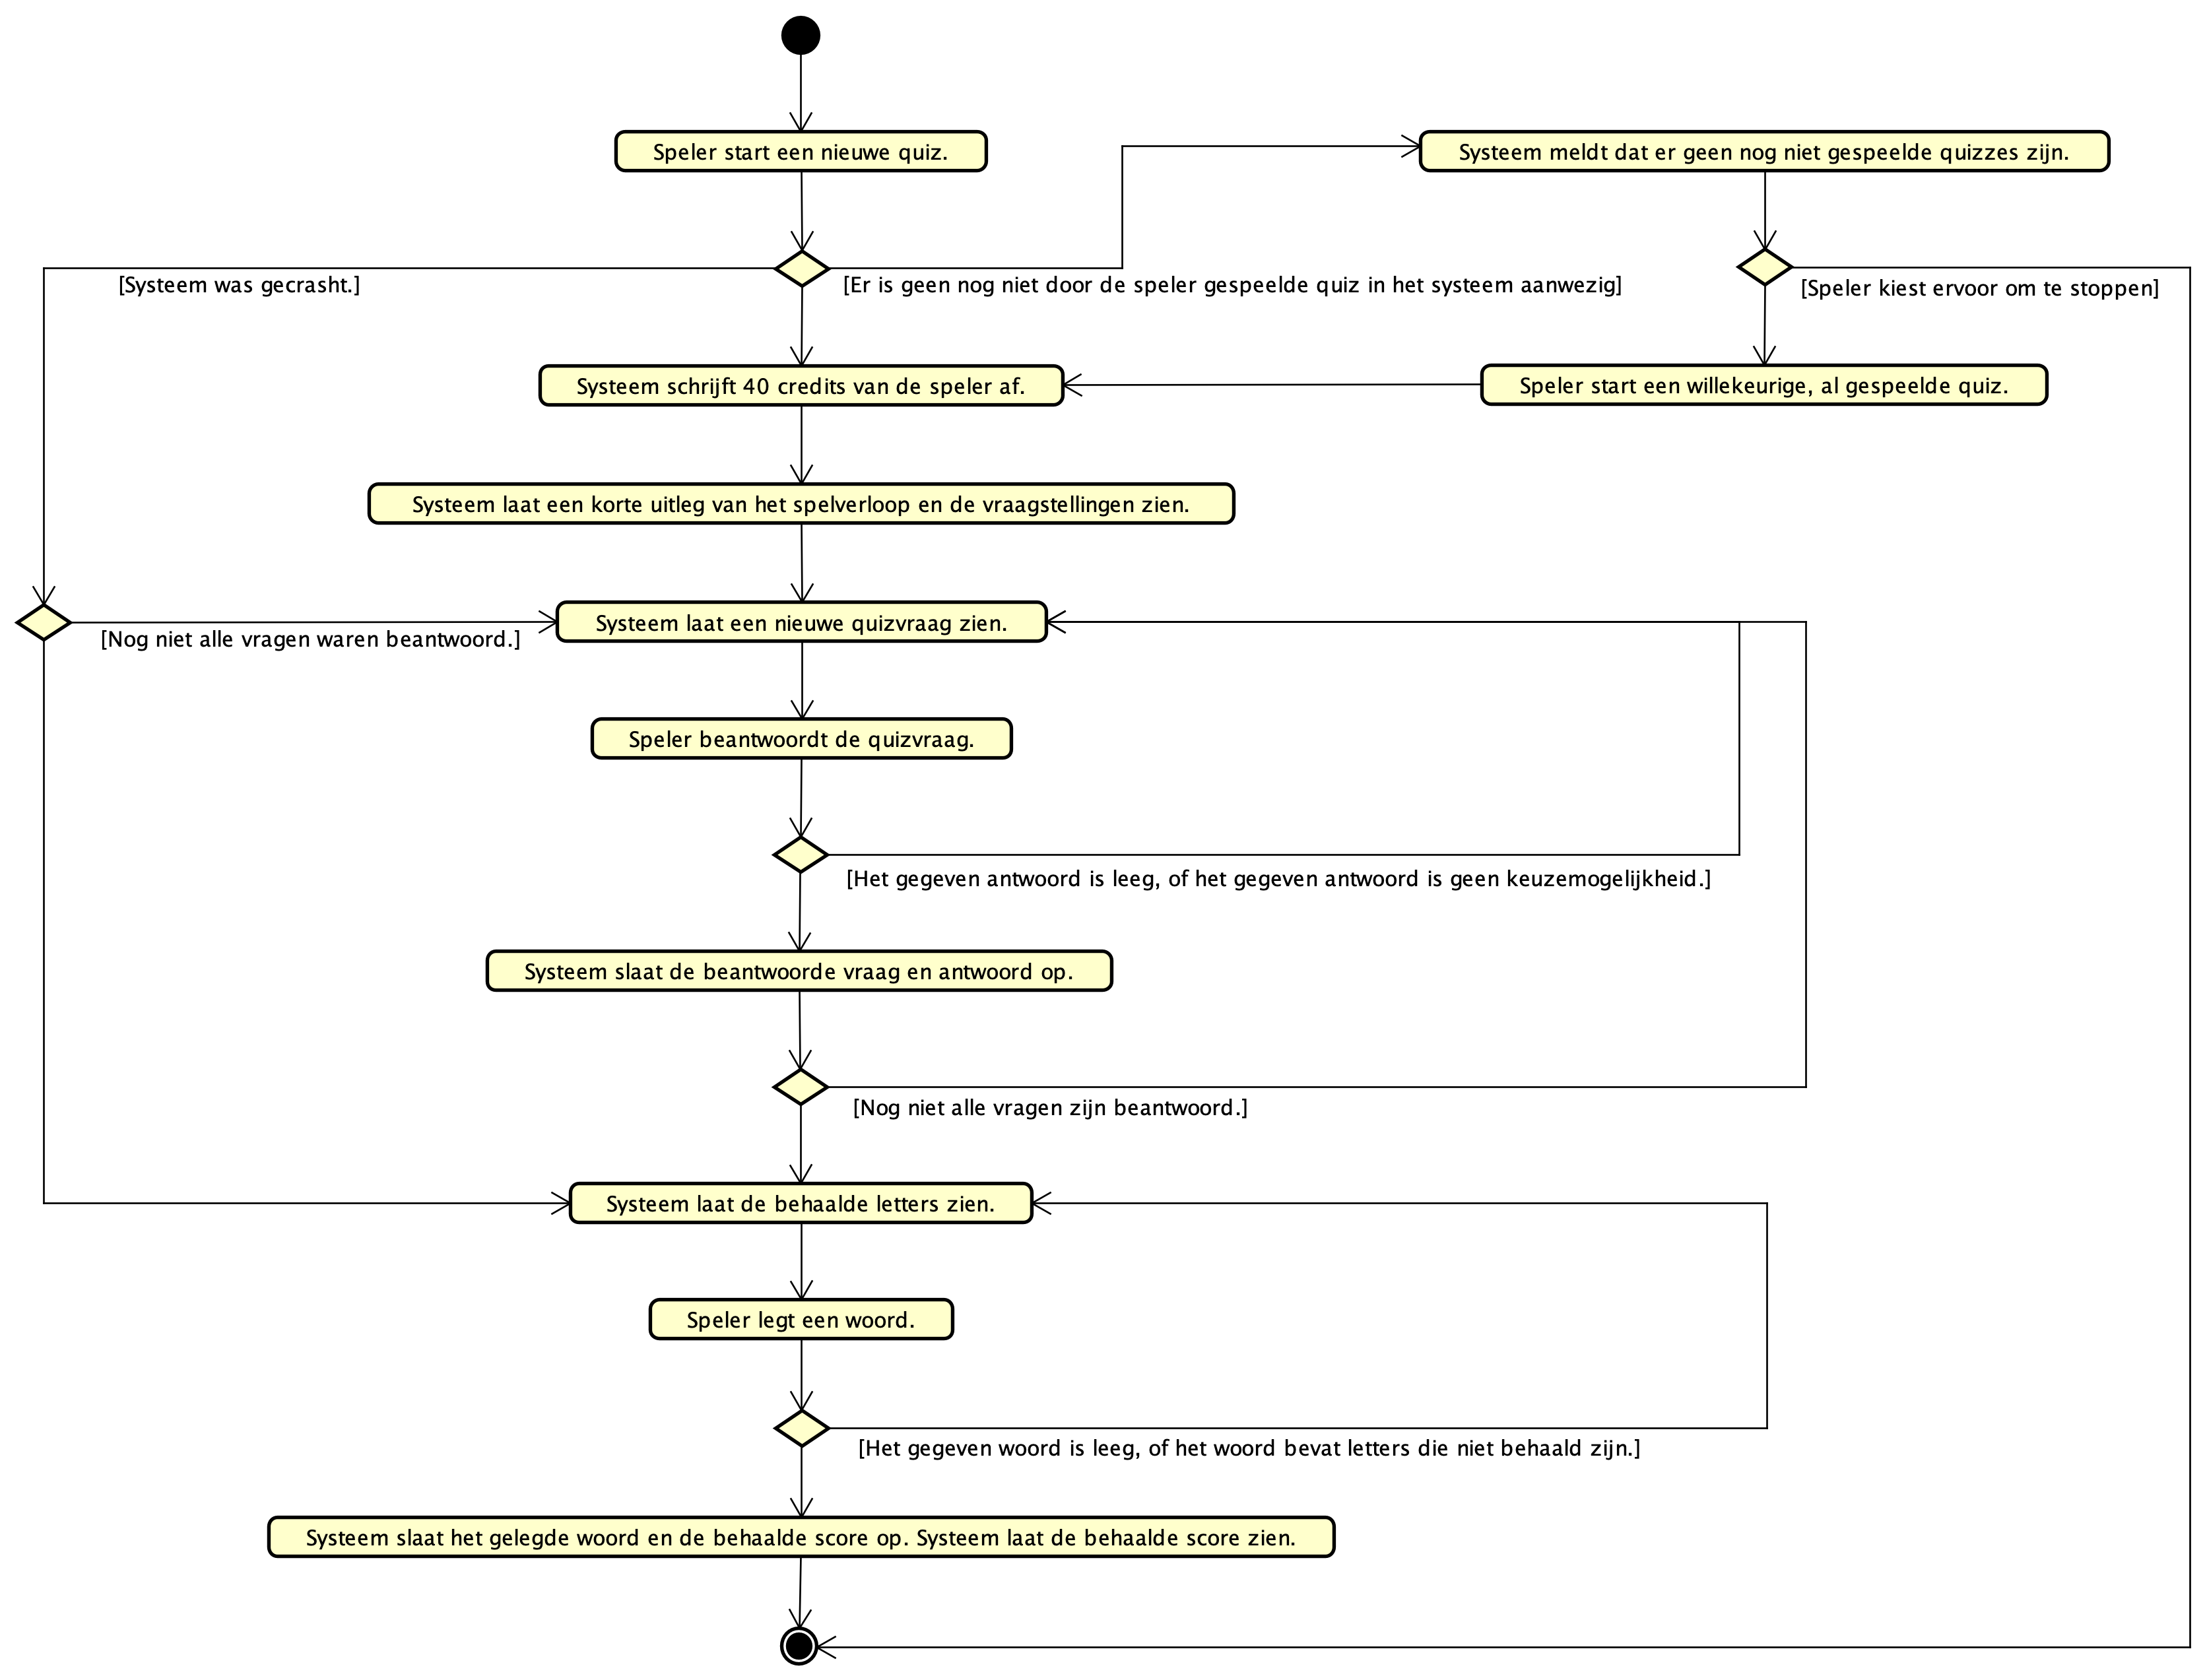
\includegraphics[width=\linewidth]{../Afbeeldingen/Quiz spelen activity diagram.png}
    \caption{Activity diagram van \textit{Quiz spelen}}
    \label{fig:activitydiagramquizspelen}
\end{mpfigure}

\label{sec:designdesicions}\subsubsection{Gemaakte ontwerpbeslissingen voor subsysteem}
%Design decisions made for subsystem <Describe all design decisions made for the sub-system. Provide at least decision descriptions for all frameworks, libraries and other technologies used. Other decisions may be related to software patterns, system-structure, adapted principles or the like.>
Het klassendiagram in figuur \ref{fig:klassendiagram} bevat een aantal beslissingen gemaakt aan de hand van een aantal design principes en patterns:

\begin{itemize}
    \item De SOLID principes in tabel \ref{tab:solid} (\cite{solid}).
    \item De Gang of Four design patterns in tabel \ref{tab:gof} (\cite[97]{designpatterns}).
    \item De GRASP principes in tabel \ref{tab:grasp} (\cite{larman}).
\end{itemize}

\begin{xltabular}{\textwidth}{p{0.2\linewidth} p{0.2\linewidth} X}
    \caption{Gebruik van de SOLID principes in het klassendiagram} \label{tab:solid} \\
    \hline\textbf{Principe} & \textbf{Plek} & \textbf{Beredenatie} \\ \hline \endfirsthead
    \hline\textbf{Principe} & \textbf{Plek} & \textbf{Beredenatie} \\ \hline \endhead
    \hline \multicolumn{3}{r}{\textit{Wordt vervolgd op de volgende pagina...}} \endfoot \endlastfoot
    Single\newline Responsibility & Quebble & Deze klasse moet alleen aan te passen zijn wanneer er usecases bijkomen. \\
    \hline
    Single\newline Responsibility & Vraag & Deze klasse moet alleen aan te passen zijn wanneer er vraagtypes bijkomen. \\
    \hline
    Single\newline Responsibility & Sco\-re\-Be\-re\-ken\-ing\-Stra\-te\-gy & Deze klasse moet alleen aan te passen zijn wanneer er strategies bijkomen. \\
    \hline
    Open-closed & Quebble & Quebble geeft slechts een aantal usecase controllers terug. Als er meer usecases bijkomen, hoeft er alleen een nieuwe controller te komen, en moet Quebble een nieuwe methode krijgen. De huidige methodes van Quebble blijven dan intact. \\
    \hline
    Open-closed & Vraag,\newline Sco\-re\-Be\-re\-ken\-ing\-Stra\-te\-gy  & Door een abstracte klasse te gebruiken is het mogelijk om nieuwe soorten ervan toe te voegen met dezelfde interface. De basisklasse heeft dan een nieuwe factory method nodig, maar de bestaande factory methods kunnen intact blijven. \\
    \hline
    Liskov\newline Substitution & Vraag & Vraag heeft als subklasses OpenVraag en MeerkeuzeVraag. De interface functioneert exact hetzelfde. Het verschil is dat de Vraag de antwoorden op een andere manier behandelt, en dat een OpenVraag altijd een lege lijst aan mogelijke antwoorden teruggeeft. Dit heeft geen invloed op een gebruiker van de API. \\
    \hline
    Interface\newline Segregation & I*Controller & Deze scheiden de publieke interface van de concrete klasse. De initialisatie van deze klasse is niet belangrijk voor de publieke API. \\
    \hline
    Interface\newline Segregation & IQuiz,\newline ISpeler,\newline IVraag & Deze scheiden de publieke interface van de concrete klasse. De concrete klassen bevatten instelmogelijkheden die alleen belangrijk zijn voor het aanmaken ervan. De repositories maken hier alleen gebruik van, de publieke API niet. \\
    \hline
    Interface\newline Segregation & I*Login* & De AuthenticatieController hoeft de Login alleen maar te beheren. De andere controllers hoeven alleen maar een huidige ISpeler op te kunnen halen. \\
    \hline
    Dependency\newline Inversion & Quiz & Quiz gebruikt de abstracte klasse ScoreBerekeningStrategy, en maakt daarbij gebruik van diens factory method. Quiz is daardoor niet afhankelijk van de concrete implementatie van de strategy. \\
    \hline
    Dependency\newline Inversion & Quiz & Quiz gebruikt de abstracte klasse Vraag. Een API neemt een lijst met abstracte Vragen aan om in te stellen als attribuut. Quiz is daardoor niet afhankelijk van de concrete implementatie ervan. \\
    \hline
    Dependency\newline Inversion & Speler & Speler gebruikt de interface IQuiz. Zijn API's nemen IQuizzes aan om in te stellen als attribuut. Speler is daardoor niet afhankelijk van de concrete implementatie van een IQuiz. \\
    \hline
    Dependency\newline Inversion & QuizBuilder & QuizBuilder gebruikt de abstracte klasse Vraag en diens factory methods. Quiz is daardoor niet afhankelijk van de concrete implementatie van de Vraag. \\
    \hline
    Dependency\newline Inversion & Quebble & Quebble maakt de Controllers aan, en retourneert de Controllers als I*Controller. De UI klasse is daardoor niet afhankelijk van de implementatie van een I*Controller. \\
    \hline

\end{xltabular}

\begin{xltabular}{\textwidth}{p{0.2\linewidth} p{0.2\linewidth} X}
    \caption{Gebruik van de Gang of Four patterns in het klassendiagram} \label{tab:gof} \\
    \hline\textbf{Pattern} & \textbf{Plek} & \textbf{Beredenatie} \\ \hline \endfirsthead
    \hline\textbf{Pattern} & \textbf{Plek} & \textbf{Beredenatie} \\ \hline \endhead
    \hline \multicolumn{3}{r}{\textit{Wordt vervolgd op de volgende pagina...}} \endfoot \endlastfoot
    Builder & QuizBuilder & Ondersteunt het bouwen van quizzes.

    Allereerst is de API van de Builder ontkoppeld door alleen maar standaard Java types te gebruiken.

    Quizzes zijn complexe objecten waarin ook Vragen aanwezig moeten zijn, en het moet mogelijk zijn om SpelStatistieken van tevoren in te stellen.

    Deze builder maakt nog een abstractielaag voor de gebruiker door instanties van IQuiz terug te geven. Dit ontkoppelt de publieke interface IQuiz van de concrete klasse (en de daarbij behorende instelmogelijkheden) Quiz. \\
    \hline
    Factory method & Sco\-re\-Be\-re\-ken\-ing\-Stra\-te\-gy & Versimpelt het gebruik van een Strategy. Wanneer de huidige strategy aan vervanging toe is, hoeft een ontwikkelaar alleen maar deze methode aan te passen. De domeinobjecten die afhankelijk zijn van de interface van een strategy, kunnen dan onveranderd blijven. \\
    \hline
    Factory method & Vraag & Ontkoppelt de interface van een Vraag van de implementaties MeerkeuzeVraag en OpenVraag. \\
    \hline
    Façade & *Controller & Ontkoppelt de voorkant van de applicatie van de domeinlaag. \\
    \hline
    Singleton & *Repository & Garandeert dat er maar één instantie is van een Repository. Dit zorgt ervoor dat er altijd één duidelijke bron is van de domeinobjecten, en versimpelt de toegang er naartoe. \\
    \hline
    Strategy & Sco\-re\-Be\-re\-ken\-ing\-Stra\-te\-gy & Maakt het makkelijk om het algoritme voor het berekenen van scores later te veranderen. \\
    \hline
\end{xltabular}

\begin{xltabular}{\textwidth}{p{0.2\linewidth} p{0.2\linewidth} X}
    \caption{Gebruik van de GRASP principes in het klassendiagram} \label{tab:grasp} \\
    \hline\textbf{Principe} & \textbf{Plek} & \textbf{Beredenatie} \\ \hline \endfirsthead
    \hline\textbf{Principe} & \textbf{Plek} & \textbf{Beredenatie} \\ \hline \endhead
    \hline \multicolumn{3}{r}{\textit{Wordt vervolgd op de volgende pagina...}} \endfoot \endlastfoot

    Creator & ConsoleUser\-Interface & ConsoleUserInterface maakt direct gebruik van Quebble. \\
    \hline
    Creator & Quebble & Quebble beschikt over de initialisatie-informatie van de Controllers, namelijk het door de Controllers gedeelde Login object. \\
    \hline
    Creator & CreditsController & CreditsController is de enige die het Betaalsysteem gebruikt. \\
    \hline
    Creator & *Repository & De repositories houden de gegevens bij van de corresponderende klassen. \\
    \hline
    Creator & Spelresultaat & Maakt direct gebruik van Score\-Berekening\-Strategy. \\
    \hline
    Creator & Quiz & Quiz beschikt over de initialisatie-informatie om SpelStatistieken te maken. Quiz gebruikt SpelStatistieken direct. \\
    \hline
    Creator & Vraag & Vragen beschikken over de intialisatie-informatie om Antwoorden te maken. Vragen gebruiken Antwoorden direct. \\
    \hline
    Controller & *Controller & De controllers zijn opgesteld als usecase controllers. De API ervan komt zoveel mogelijk overeen met de stappen uit de bijbehorende usecases (zie Software Requirements Specification). \\
    \hline
    Expert & Quiz & Quiz kan de Spelstatistieken bijhouden omdat hij weet welke Vragen er zijn, kan tellen hoeveel Vragen er goed zijn, en de uitslag van de goedkeuring van het gelegde Woord kan opvragen. \\
    \hline
    Expert & * & Op alle onderstaande plekken waar indirection is toegepast, is die klasse ook de information expert voor alle API's waar hij bemiddelt tussen onderliggende domeinobjecten. \\
    \hline
    High Cohesion & Vraag & Alle Vraag- en Antwoord klassen zijn heel samenhangend, en het enige toegangspunt als API is hiervoor IVraag. \\
    \hline
    Indirection & QuizBuilder & Gebruikt standaard Java types als API, en handelt het maken van quizzes met bijbehorende vragen af. \\
    \hline
    Indirection & *Controller & De controllers zijn façade klassen, en gebruiken enkel standaard Java types als API om de koppeling tussen de domeinlaag en de servicelaag zo los mogelijk te houden. De controllers regelen dan ook de interactie tussen domeinobjecten, zodat deze los gekoppeld blijven. \\
    \hline
    Indirection & IQuiz & De interface IQuiz gebruikt alleen maar standaard Java types als API, en handelt de interactie tussen zichzelf, Vragen, Woord, SpelStatistieken en Spelresultaat af. \\
    \hline
    Indirection & Woord & De API gebruikt alleen maar standaard Java types, en Woord handelt de interactie tussen zichzelf en Letters af. \\
    \hline
    Indirection & Vraag & De API gebruikt alleen maar standaard Java types, en Vraag handelt de interactie tussen zichzelf en bijbehorende Antwoorden af. \\
    \hline
    Low Coupling & * & Alle klassen die Indirection toepassen dragen bij aan een lage koppeling tussen objecten. \\
    \hline
    Polymorphism & Vraag & MeerkeuzeVragen en OpenVragen gaan anders om met het goedkeuren van antwoorden, en met het laten zien van mogelijke antwoorden. \\
    \hline
    Polymorphism & Sco\-re\-Be\-re\-ken\-ing\-Stra\-te\-gy & Is uitbreidbaar met meerdere factory methods om verschillende varianten aan te bieden. \\
    \hline
    Pure fabrication & *Repository & Zijn geen onderdeel van het domein, dienen alleen als persistentie hulpmiddel. \\
    \hline
    Pure fabrication & *Controller,\newline Quebble & Zijn geen onderdeel van het domein, dienen als API voor de voorkant van de applicatie. \\
    \hline
    Pure fabrication & QuizBuilder & Is geen onderdeel van het domein, dient als hulpmiddel om het bouwen van Quiz-objecten te versimpelen. \\
    \hline
    Pure fabrication & *Login* & Is geen onderdeel van het domein, dient als hulpmiddel om de huidig ingelogde speler bij te houden of aan te passen. \\
    \hline
    Pure fabrication & Console\-User\-Interface & Is geen onderdeel van het domein, dient als startpunt en UI voor de applicatie. \\
    \hline
    Pure fabrication & Stopwatch & Is geen onderdeel van het domein, dient als hulpmiddel om de gespeelde tijd bij te houden. \\
    \hline
\end{xltabular}

%\subsection{Design subsystem B (and so on)}

%\subsection{Databaseontwerp}
%Database design <. If your system uses relational databases, make sure you provide a physical datamodel here.> 

%\subsubsection{Database gerelateerde ontwerpbeslissingen}
%Design decisions related to the database <Describe all design decisions made along the database. This could include the choice of the database management system, the use of  certain triggers or stored procedures, special indexes and so on.>

\clearpage\printbibliography[heading=bibintoc]

\end{document}